\documentclass[12pt]{article}
\usepackage{fullpage,enumitem,amsmath,amssymb,graphicx}

\begin{document}

\begin{center}
{\Large CS221 Fall 2018 Homework [scheduling]}

\begin{tabular}{rl}
SUNet ID: & prabhjot \\
Name: & Prabhjot Singh Rai
\end{tabular}
\end{center}

By turning in this assignment, I agree by the Stanford honor code and declare
that all of this is my own work.

\section*{Problem 0}

\begin{enumerate}[label=(\alph*)]
  \item The problem statement can be visualised as below: \\
  \begin{center}
  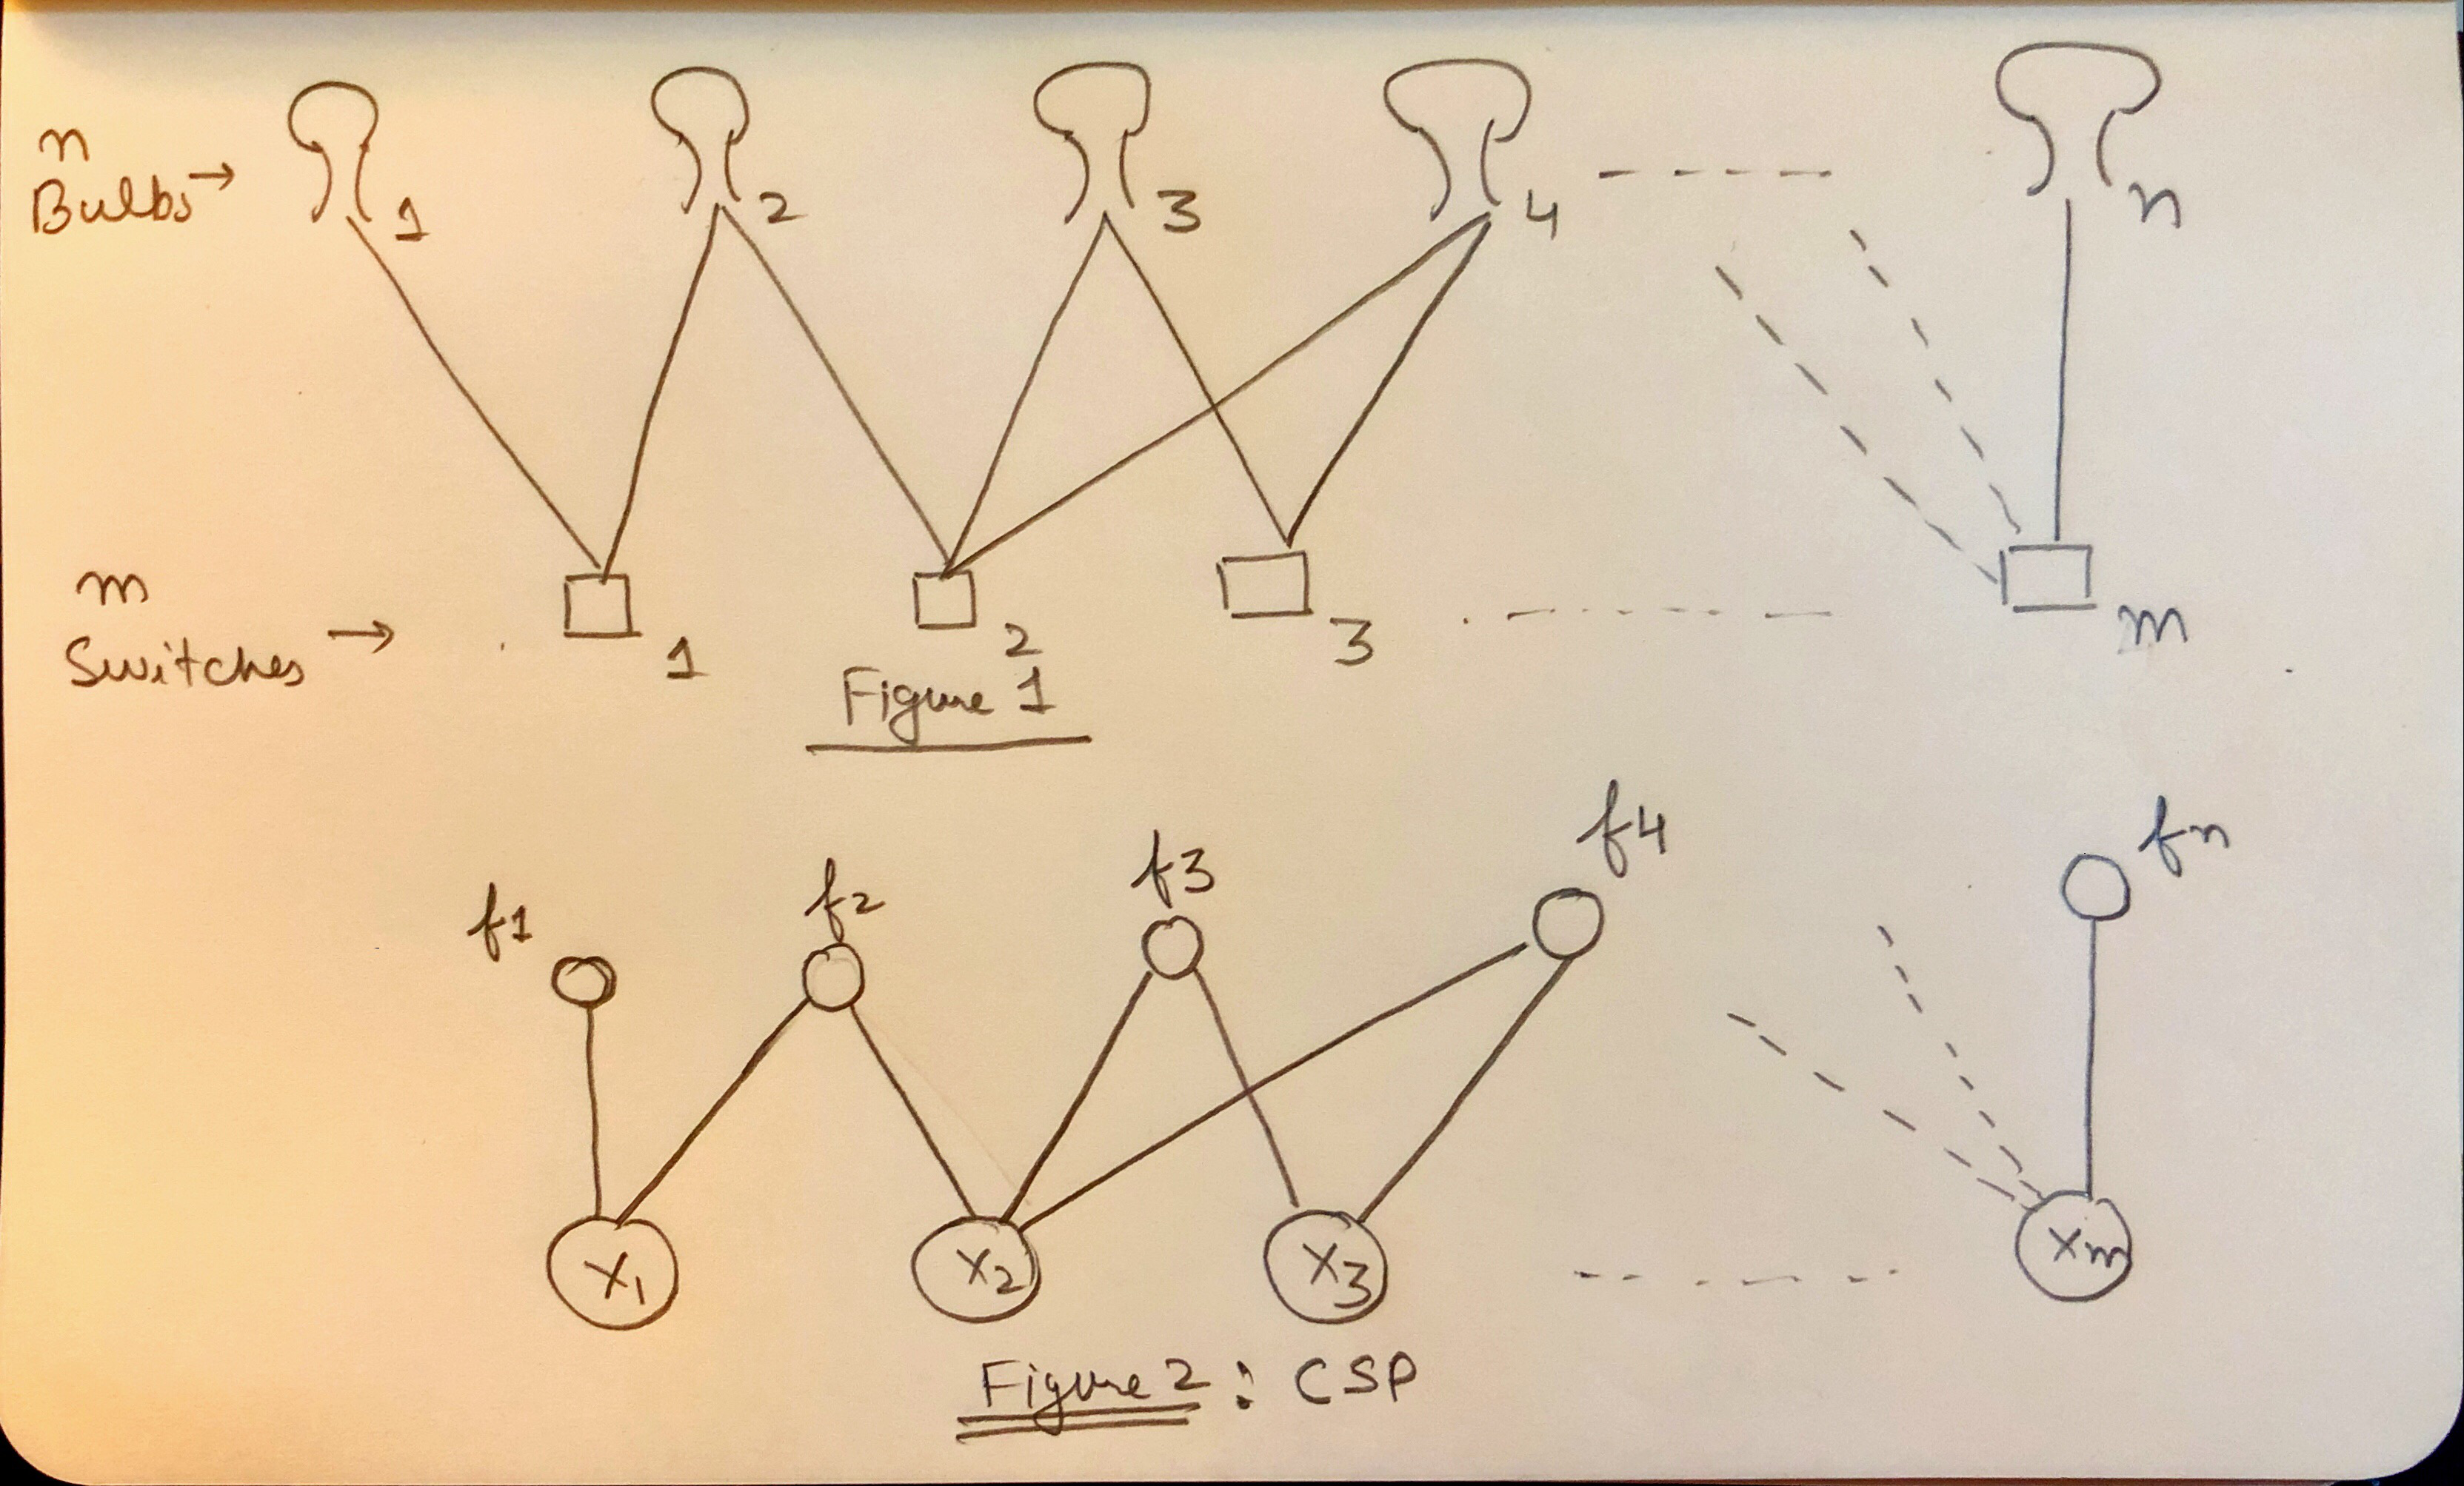
\includegraphics[scale=0.1]{IMG_2239.png}
  \end{center}
  \textbf{Variables}: The variables for the CSP are the m switches, $X_1, X_2 ... X_m$. The domain of these variables are Domains $   \epsilon \{0, 1\}$, $0$ being the "off" state for a switch and $1$ being the "on" state. \\
  \textbf{Constraints}: The constraints or the factors are created among a bulb and it's controlling switch(es). For example, from above Figure 1, if switch 1 controls bulb 1 and bulb 2, and switch 2 controls bulb 2 and bulb 3, a factor corresponding to bulb 1 would have switch 1 value as it's parameter (be dependent on switch 1) and bulb 2 would have values of both switch 1 and switch 2 as it's parameters. Since $T_j$ (for each button $j=1, ...m$) defines every set of light bulbs a switch controls, factor $f_k$ (for each light bulb $k=1,...n$) would depend on variable $j$ if $k$ in $T_j$. The value of this factor should return an odd number, so that even numbers render the state of the bulb to be "off" and last number makes the bulb "on".
  \begin{align*}
  f_k (X_1[\text{$k$ in $T_1$}], & X_2[\text{$k$ in $T_2$}], ... X_m[\text{$k$ in $T_m$}]) \\ & = sum(X_1[\text{$k$ in $T_1$}], X_2[\text{$k$ in $T_2$}], ... X_m[\text{$k$ in $T_m$}]) \% 2 == 1
  \end{align*}
  \item
  \begin{enumerate}
  \item For finding consistent assignments, we draw the table for finding values of $t_1$ and $t_2$. From the Table 1, we can see that there are two consistent solutions for $x_1, x_2, x_3$, one being $\{0, 1, 0 \}$ and other being $\{ 1, 0, 1\}$, respectively.
  \begin{table}
\centering
\caption{Table depicting unigram costs assigned to words}
\begin{tabular}{|l|l|l|l|l|l|} 
\hline
x1 & x2 & x3 & t1(x) & t2(x) & \textbf{Consistency}  \\ 
\hline
0  & 0  & 0  & 0       & 0       & 0                     \\ 
\hline
0  & 0  & 1  & 0       & 1       & 0                     \\ 
\hline
0  & 1  & 0  & 1       & 1       & 1                     \\ 
\hline
0  & 1  & 1  & 1       & 0       & 0                     \\ 
\hline
1  & 0  & 0  & 1       & 0       & 0                     \\ 
\hline
1  & 0  & 1  & 1       & 1       & 1                     \\ 
\hline
1  & 1  & 0  & 0       & 1       & 0                     \\ 
\hline
1  & 1  & 1  & 0       & 0       & 0                     \\
\hline
\end{tabular}
\end{table}
  \end{enumerate}
  \item For fixed variables $X_1, X_2, X_3$, backtrack will be called in following ways:
  \begin{align*}
  backtrack(\phi, 1, \{x_1: [0, 1], x_2: [0, 1], x_3: [0,1]\}) \\
  backtrack(\{x_1: 0\}, 1, \{x_1: [0, 1], x_2: [0, 1], x_3: [0,1]\}) \\
  backtrack(\{x_1: 0, x_3: 0\}, 1, \{x_1: [0, 1], x_2: [0, 1], x_3: [0,1]\}) \\
  backtrack(\{x_1: 0, x_2: 1, x_3: 0\}, 1, \{x_1: [0, 1], x_2: [0, 1], x_3: [0,1]\}) \\
  backtrack(\{x_1: 0, x_3: 1\}, 1, \{x_1: [0, 1], x_2: [0, 1], x_3: [0,1]\}) \\
  backtrack(\{x_1: 1\}, 1, \{x_1: [0, 1], x_2: [0, 1], x_3: [0,1]\}) \\
  backtrack(\{x_1: 1, x_3: 0\}, 1, \{x_1: [0, 1], x_2: [0, 1], x_3: [0,1]\}) \\
  backtrack(\{x_1: 1, x_3: 1\}, 1, \{x_1: [0, 1], x_2: [0, 1], x_3: [0,1]\}) \\
  backtrack(\{x_1: 1, x_2: 0, x_3: 1\}, 1, \{x_1: [0, 1], x_2: [0, 1], x_3: [0,1]\})
  \end{align*}
  Therefore, backtrack algorithm is called 9 times.
  \item When lookahead is enabled (AC3):
  \begin{align*}
  backtrack(\phi, 1, \{x_1: [0, 1], x_2: [0, 1], x_3: [0,1]\}) \\
  backtrack(\{x_1: 0\}, 1, \{x_1: [0], x_2: [1], x_3: [0]\}) \\
  backtrack(\{x_1: 0, x_3: 0\}, 1, \{x_1: [0], x_2: [1], x_3: [0]\}) \\
  backtrack(\{x_1: 0, x_2: 1 x_3: 0\}, 1, \{x_1: [0], x_2: [1], x_3: [0]\}) \\
  backtrack(\{x_1: 1\}, 1, \{x_1: [1], x_2: [0], x_3: [1]\}) \\
  backtrack(\{x_1: 1, x_3: 1\}, 1, \{x_1: [1], x_2: [0], x_3: [1]\}) \\
  backtrack(\{x_1: 1, x_2: 0 x_3: 1\}, 1, \{x_1: [1], x_2: [0], x_3: [1]\})
  \end{align*}
  Therefore, backtrack algorithm with AC3 is called 7 times.
\end{enumerate}
\section*{Problem 2}

\begin{enumerate}[label=(\alph*)]
  \item (your solution)
  \item (your solution)
\end{enumerate}

\end{document}